\chapter{Validation croisée des simulations}
Dans cette section, par souci de simplicité, juste les sous-systèmes avec la configuration finale est exploré. 

\section{Convertisseur CC-CC 4 quadrants formé de 2 convertisseurs 3 niveaux NPC}
Ce sous-système représente le DCP/DCN, le convertisseur CC-CC indiqué sur la figure présenté au début de ce document représentant le schéma complet du système à implémenter. Le fonctionnalité de ce système est de reproduire une forme de courant précise à la charge, il est testé sur source idéal et est capable de  reproduire le courant désirée sur une charge RL comme on le remarque sur la figure~\ref{DC_ch_cou_1}, il n'y a pas de grosse différence entre PSIM et SPS mise à part un décalage en fréquence. La dynamique du système suit très bien la courbe de référence avec une oscillation d'environs 15A. Il y a présence de commutation non désirée mais ça n'affecte pas le fonctionnement du système. 



\begin{figure}[htb]
\centering
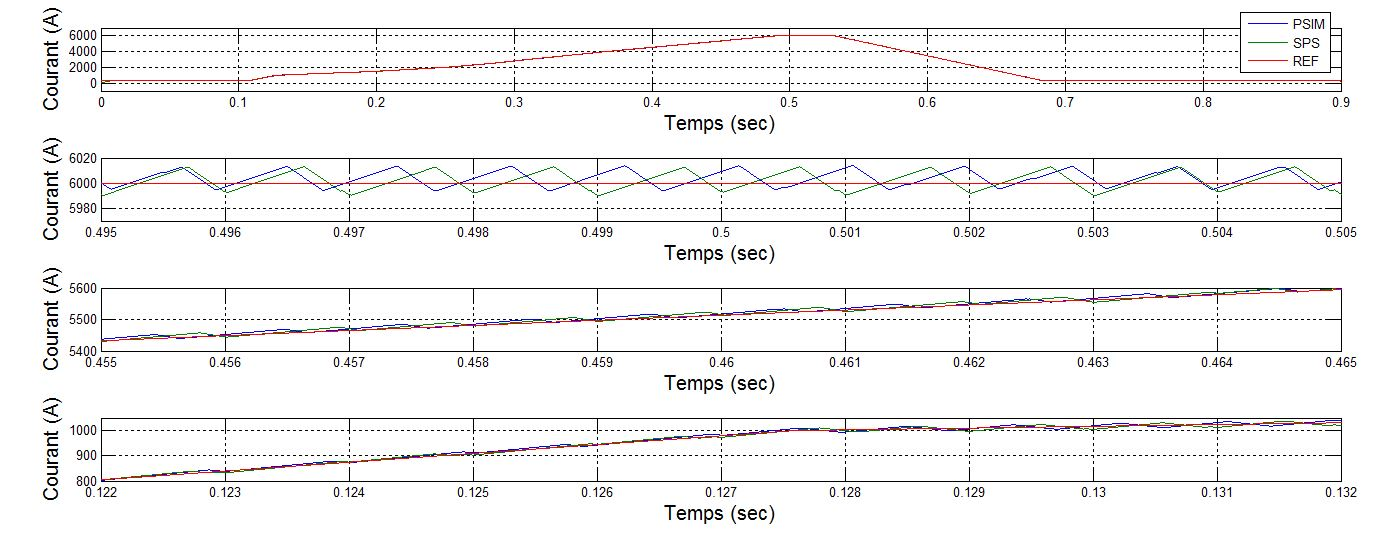
\includegraphics[scale=0.5]{fig/DCPDCN/DCPCourantCharge1u.jpg}
\caption{Courant traversant la charge sur PSIM et SPS pour un pas de calcul de 1$\mu$s pour le DCP/DCN}
\label{DC_ch_cou_1}
\end{figure}

\begin{figure}[htb]
\centering
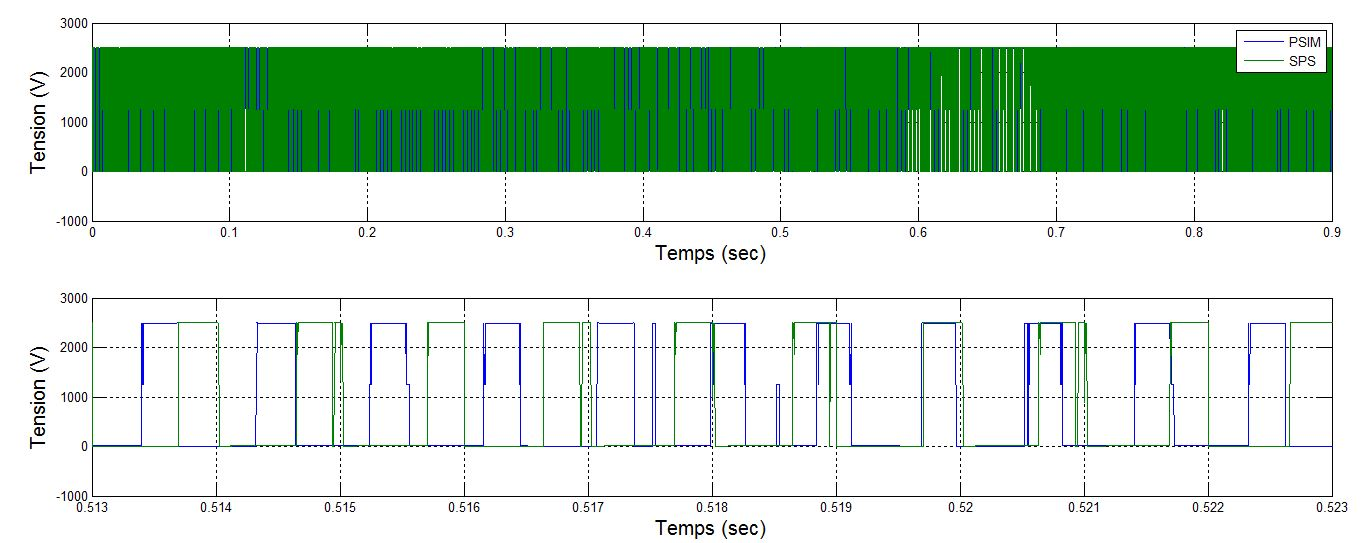
\includegraphics[scale=0.5]{fig/DCPDCN/DCPTensionIGBT1u.jpg}
\caption{Tension aux bornes d'un IGBT sur PSIM et SPS pour un pas de calcul de 1$\mu$s pour le DCP/DCN}
\label{DC_IG_ten_1}
\end{figure}

\clearpage
\section{AFE 3 niveaux NPC avec contrôle par MLI}
Ce sous-système représente l'AFE. Il est testée sur une consigne de tension périodique pour reproduire la dynamique du système. La figure~\ref{AF_RC_cou} montre que le système réagit au changement de consigne de courant de manière identique entre PSIM et SPS. On remarque un décalage entre la courbe de tension de PSIM et SPS tel que vu sur la figure~\ref{AF_RC_ten} d'environs 5V. Dû au nombre élevé de complexité du modèle il est difficile d'indiquer exactement ce qui peut causer cette différence mais on remarque de même un fonctionnement pratiquement identique entre PSIM et SPS. On observe sur la figure~\ref{AF_RC_igbt} que les commutation de SPS et PSIM sont identiques et se déroulent au même moment.


\begin{figure}[htb]
\centering
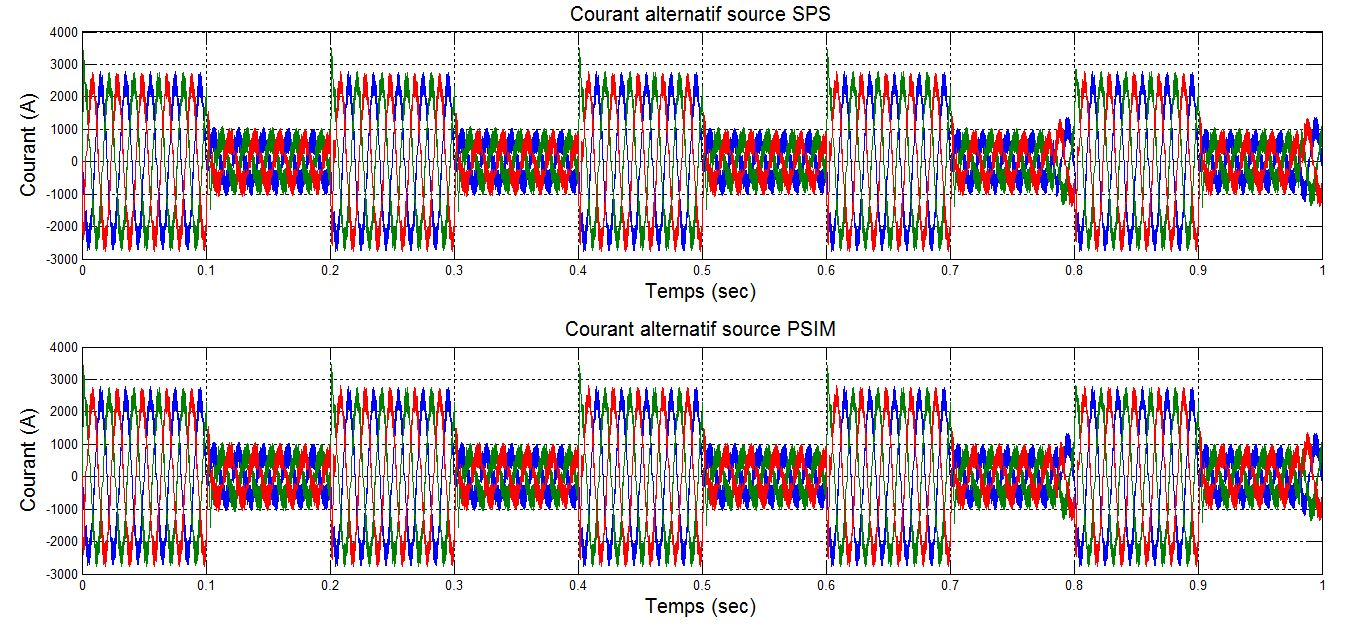
\includegraphics[scale=0.5]{fig/coual_afe.jpg}
\caption{Le courant d'entré à 1$\mu$s pour l'AFE sur charge RC}
\label{AF_RC_cou}
\end{figure}




\begin{figure}[htb]
\centering
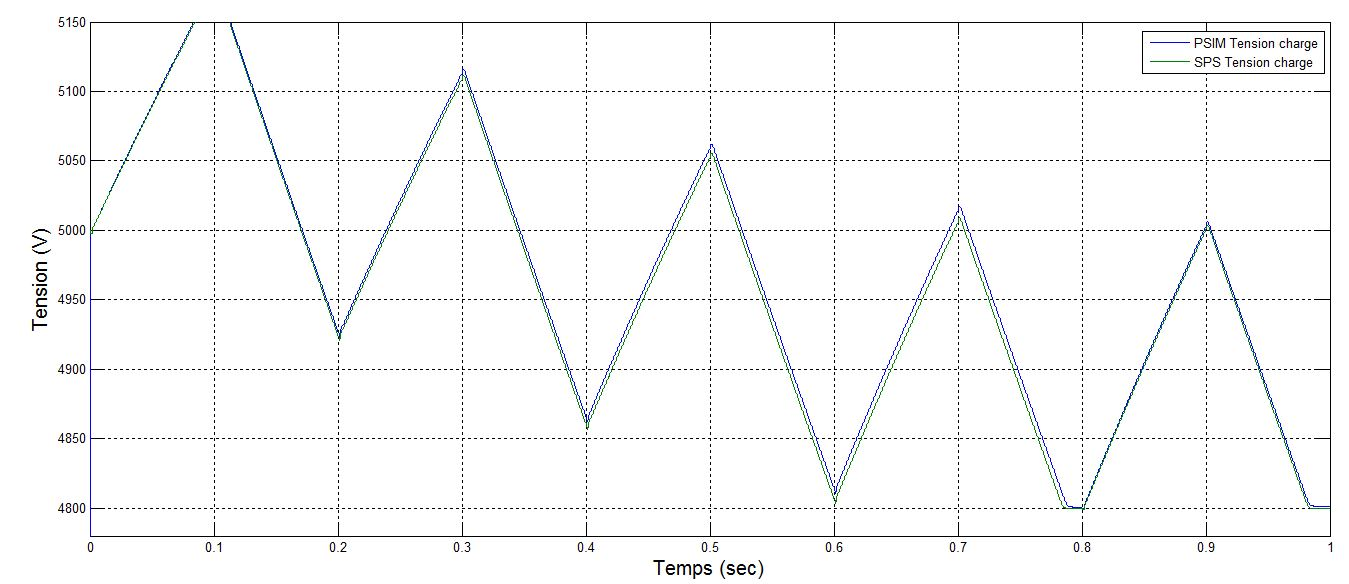
\includegraphics[scale=0.5]{fig/ten_afe.jpg}
\caption{La tension à la charge à 1$\mu$s pour l'AFE sur charge RC}
\label{AF_RC_ten}
\end{figure}



\begin{figure}[htb]
\centering
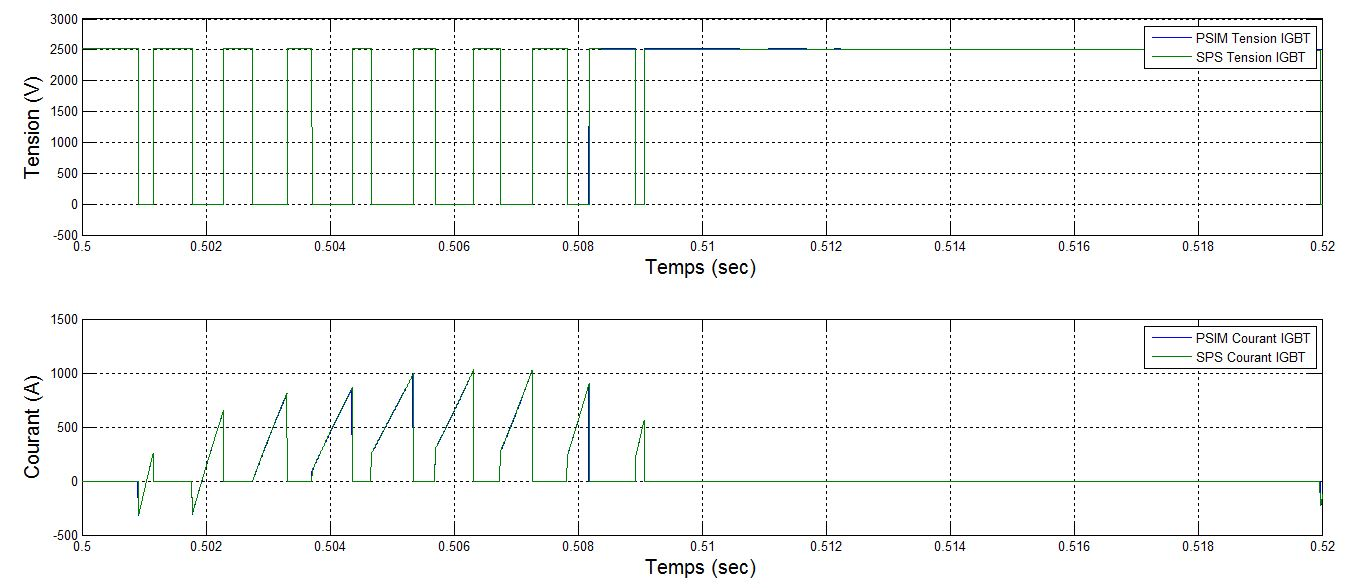
\includegraphics[scale=0.5]{fig/com_afe.jpg}
\caption{La tension et le courant au bornes d'un IGBT à 1$\mu$s pour l'AFE sur charge RC}
\label{AF_RC_igbt}
\end{figure}

\clearpage
\section{AFE 3 niveaux NPC avec contrôle par MLI avec convertisseur CC-CC formé de 2 cellules NPC 3 niveaux}
Ce sous-système représente le système complet, l'intégration de l'AFE et le DCP/DCN. On observe un fonctionnement tout à fait semblable mise à part un décalage d'environs 50V entre PSIM et SPS tel que vu sur la figure~\ref{AF_DC_vch1}. On observe que pour les deux systèmes, soit SPS et PSIM, on arrive à 200V environs de la courbe obtenu par le CERN au niveau de la tension sur le bus CC. Cette différence s'explique par un manque de donnée et d'information par rapport au système complet du CERN. Malgré un manque de donnée, nous réussissons à reproduire la forme de courant désirée~\ref{AF_DC_CHA1}. Une oscillation d'environs 15A est aperçu. Par contre, même si on réussi à limiter la puissance active délivrée du réseau à 3.6MW tel que montré sur la figure~\ref{AF_DC_CHA2}. On observe que PSIM délivre une puissance on peu plus élevé de SPS ce qui fait en sorte que le bus CC finit de se recharger environs 30ms avant sur PSIM que SPS.


\begin{figure}[htb]
\centering
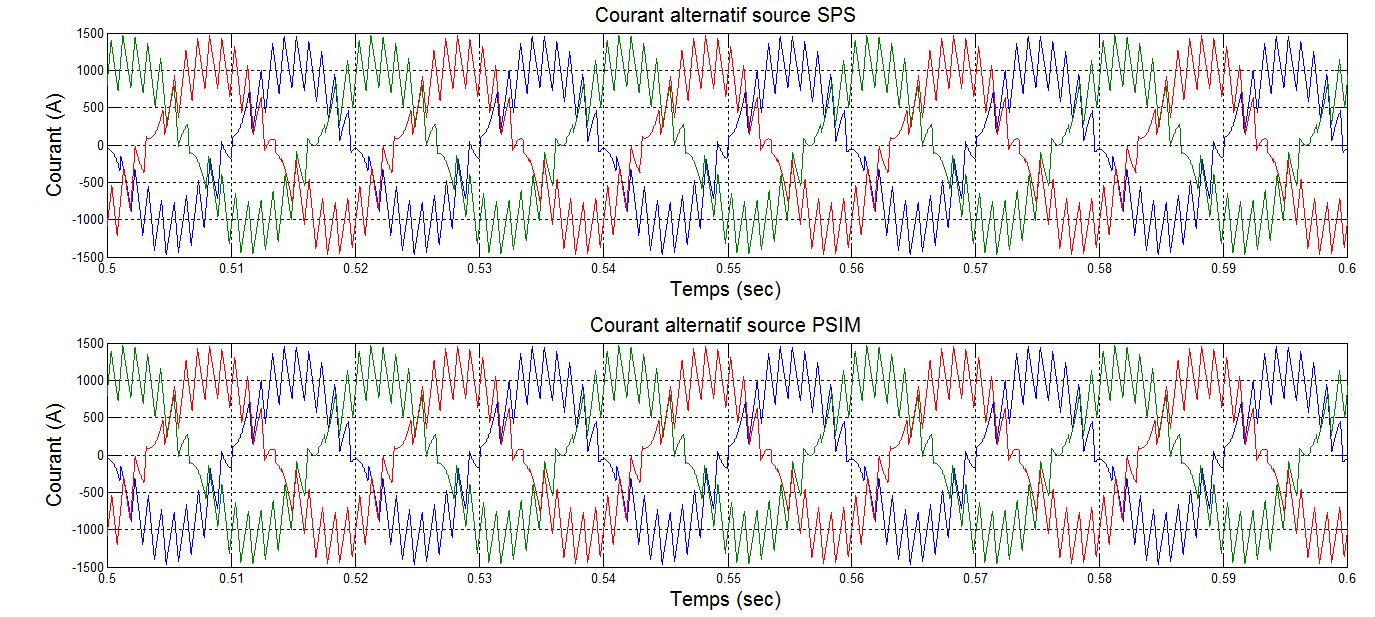
\includegraphics[scale=0.5]{fig/DCP_AFE/1u/cour_al.jpg}
\caption{Le courant d'entrée de l'AFE pour un pas de calcul de 1$\mu$s}
\label{AF_DC_cou1}
\end{figure}


\begin{figure}[htb]
\centering
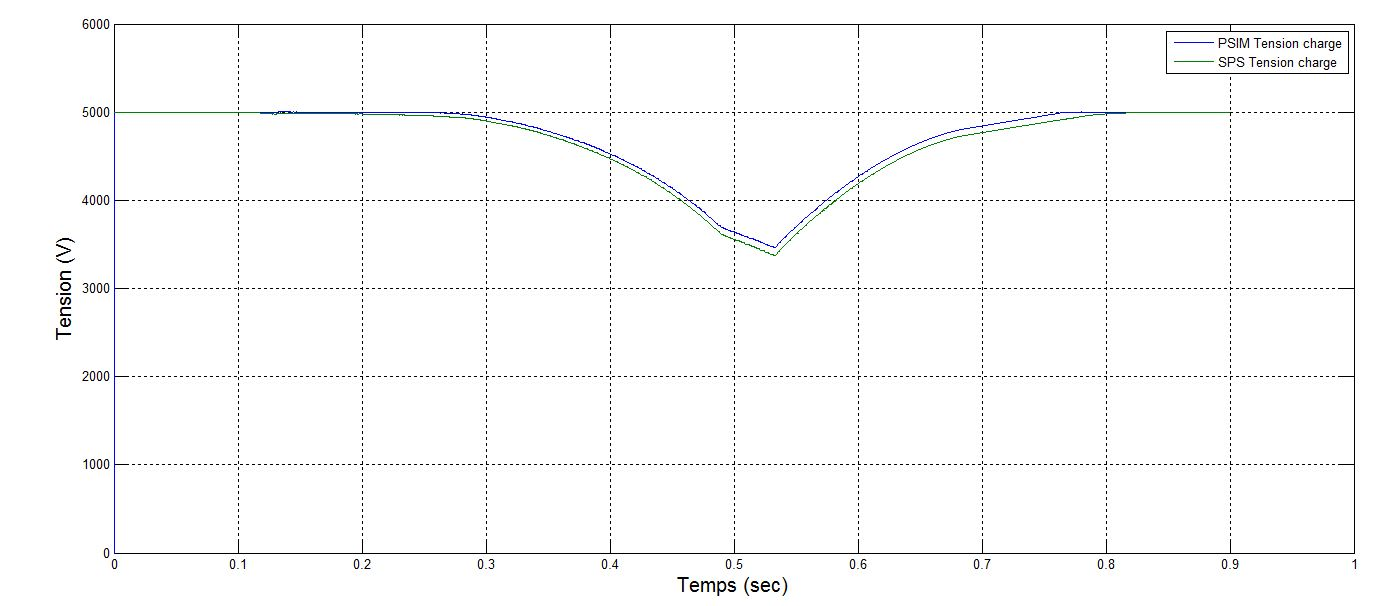
\includegraphics[scale=0.5]{fig/DCP_AFE/1u/ten_bus.jpg}
\caption{La tension du bus CC pour un pas de calcul de 1$\mu$s}
\label{AF_DC_vch1}
\end{figure}

\begin{figure}[htb]
\centering
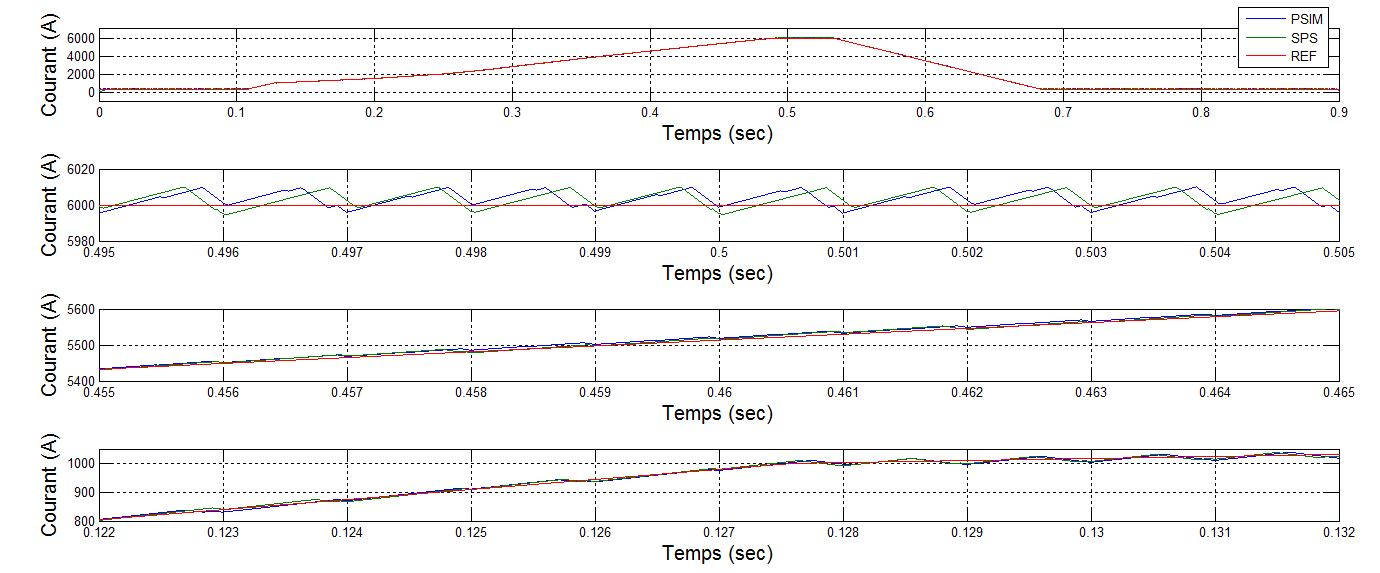
\includegraphics[scale=0.5]{fig/DCP_AFE/1u/cour_ch.jpg}
\caption{Le courant aux bornes des électroaimants pour un pas de calcul de 1$\mu$s}
\label{AF_DC_CHA1}
\end{figure}

\begin{figure}[htb]
\centering
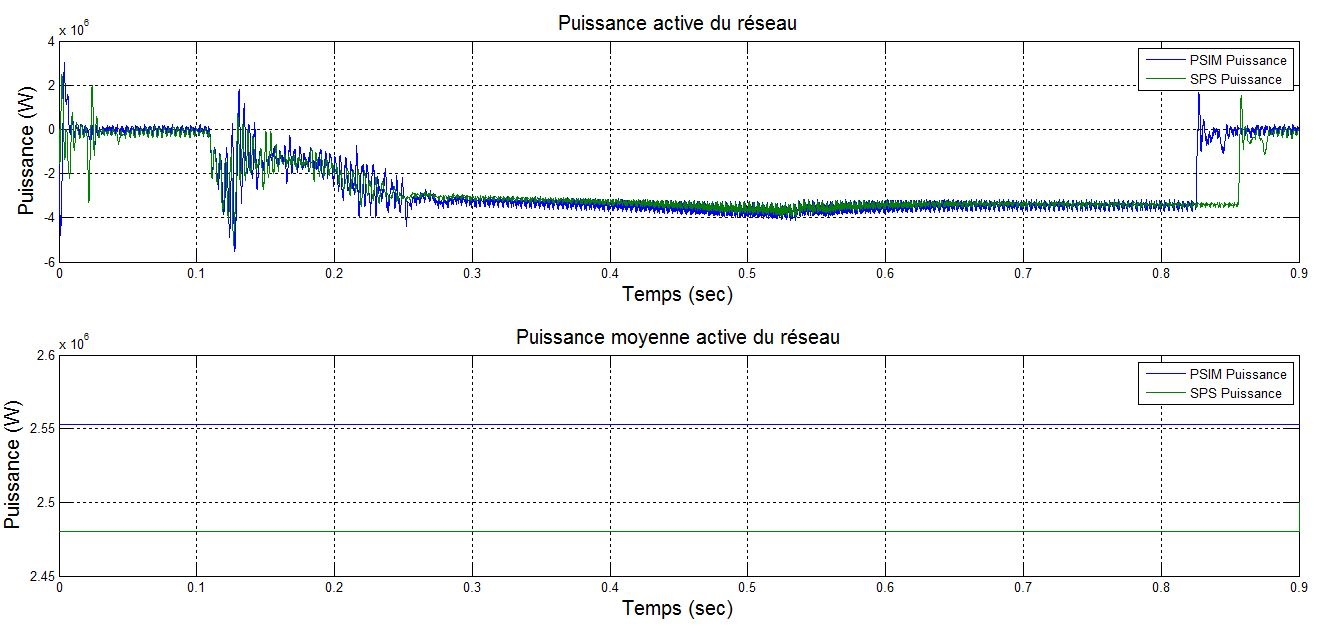
\includegraphics[scale=0.5]{fig/DCP_AFE/1u/PUI.jpg}
\caption{La puissance délivrée par le réseau alternatif pour un pas de calcul de 1$\mu$s}
\label{AF_DC_CHA2}
\end{figure}


